\testfile{pgfplotstest.axislines.tex}

\long\def\AXISLINETESTS#1{

\testsection{Axislines placement -- #1}

\def\smallplotstestyoffset{%
\addplot[smooth,blue,mark=*] coordinates {
	(-1,	11)
	(-0.75,	10.5625)
	(-0.5,	10.25)
	(-0.25,	10.0625)
	(0,		10)
	(0.25,	10.0625)
	(0.5,	10.25)
	(0.75,	10.5625)
	(1,		11)
};
}

\def\smallplotstestyoffsetneg{%
\addplot[smooth,blue,mark=*] coordinates {
	(-1,	-11)
	(-0.75,	-10.5625)
	(-0.5,	-10.25)
	(-0.25,	-10.0625)
	(0,		-10)
	(0.25,	-10.0625)
	(0.5,	-10.25)
	(0.75,	-10.5625)
	(1,		-11)
};
}

\def\smallplotstestxoffset{%
\addplot[smooth,blue,mark=*] coordinates {
	(9,	1)
	(9.25,	0.5625)
	(9.5,	0.25)
	(9.75,	0.0625)
	(10,		0)
	(10.25,	-0.0625)
	(10.5,	-0.25)
	(10.75,	-0.5625)
	(11,		-1)
};
}

\def\smallplotstestxoffsetneg{%
\addplot[smooth,blue,mark=*] coordinates {
	(-9,	1)
	(-9.25,	0.5625)
	(-9.5,	0.25)
	(-9.75,	0.0625)
	(-10,		0)
	(-10.25,	-0.0625)
	(-10.5,	-0.25)
	(-10.75,	-0.5625)
	(-11,		-1)
};
}

\testsubsection{tick align=outside}
\begin{tikzpicture}
\begin{axis}[
	tick align=outside,
	]
	\smallplotstest
\end{axis}
\end{tikzpicture}

\testsubsection{#1 -- axis y line/ axis x line}
\begin{tikzpicture}
\begin{axis}[
	axis y line=center,
	axis x line=bottom
	]
	\smallplotstest
\end{axis}
\end{tikzpicture}

\testsubsection{#1 -- axis [xy] line/ tick align/ y discont}
\begin{tikzpicture}
\begin{axis}[
	axis y discontinuity=crunch,
	axis y line=center,
	axis x line=bottom,
	tick align=center,
	%ymin=9
	]
	\smallplotstestyoffset
\end{axis}
\end{tikzpicture}

\testsubsubsection{#1 -- box / middle}
\begin{tikzpicture}
\begin{axis}[
	enlargelimits=false,
	minor tick num=3,
	axis y line=box,
	axis x line=middle
	]
	\addplot[blue,mark=none] plot[id=sinneg,domain=-10:0,samples=40] function{sin(x)};
\end{axis}
\end{tikzpicture}

\testsubsubsection{#1 -- left / middle}
\begin{tikzpicture}
\begin{axis}[
	enlargelimits=false,
	minor tick num=3,
	axis y line=left,
	axis x line=middle
	]
	\addplot[blue,mark=none] plot[id=sinneg,domain=-10:0,samples=40] function{sin(x)};
\end{axis}
\end{tikzpicture}

\testsubsubsection{#1 -- right / middle}
\begin{tikzpicture}
\begin{axis}[
	enlargelimits=false,
	minor tick num=3,
	axis y line=right,
	axis x line=middle
	]
	\addplot[blue,mark=none] plot[id=sinneg,domain=-10:0,samples=40] function{sin(x)};
\end{axis}
\end{tikzpicture}

\testsubsubsection{#1 -- center / box}
%\tracingmacros=2\tracingcommands=2
\begin{tikzpicture}
\begin{axis}[
	enlargelimits=false,
	minor tick num=3,
	axis y line=center,
	axis x line=box,
	ymin=0, ymax=25
	]
	\addplot[blue,mark=none] plot[id=sinneg,domain=-5:5,samples=40] function{x*x+1};
\end{axis}
\end{tikzpicture}

\testsubsubsection{#1 -- center / top}
\begin{tikzpicture}
\begin{axis}[
	enlargelimits=false,
	minor tick num=3,
	axis y line=center,
	axis x line=top,
	ymin=0, ymax=25
	]
	\addplot[blue,mark=none] plot[id=sinneg,domain=-5:5,samples=40] function{x*x+1};
\end{axis}
\end{tikzpicture}

\testsubsubsection{#1 -- center / bottom}
\begin{tikzpicture}
\begin{axis}[
	enlargelimits=false,
	minor tick num=3,
	axis y line=center,
	axis x line=bottom,
	ymin=0, ymax=25
	]
	\addplot[blue,mark=none] plot[id=sinneg,domain=-5:5,samples=40] function{x*x+1};
\end{axis}
\end{tikzpicture}

\testsubsubsection{#1 -- center / middle}

\begin{tikzpicture}
\begin{axis}[
	enlargelimits=false,
	minor tick num=3,
	axis y line=center,
	axis x line=middle
	]
	\addplot[blue,mark=none] plot[id=sinneg,domain=-5:5,samples=40] function{sin(x)};
\end{axis}
\end{tikzpicture}






\testsubsection{#1 -- axis [xy] line/ tick align/ x discont}
\testsubsubsection{#1 - middle/box parallel}
\begin{tikzpicture}
\begin{axis}[
	axis y line=box,
	axis x discontinuity=parallel,
	axis x line=middle,
	tick align=outside,
	xmin=8.5
	]
	\smallplotstestxoffset
\end{axis}
\end{tikzpicture}

\testsubsubsection{#1 - middle/box parallel (2)}
\begin{tikzpicture}
\begin{axis}[
	axis y line=box,
	axis x discontinuity=parallel,
	axis x line=middle,
	tick align=outside,
	]
	\smallplotstestxoffsetneg
\end{axis}
\end{tikzpicture}

\testsubsubsection{#1 - middle/box crunch}
\begin{tikzpicture}
\begin{axis}[
	axis y line=box,
	axis x discontinuity=crunch,
	axis x line=middle,
	tick align=outside,
	]
	\smallplotstestxoffset
\end{axis}
\end{tikzpicture}


\testsubsubsection{#1 - middle/box crunch parallel}
\begin{tikzpicture}
\begin{axis}[
	axis y line=box,
	axis x discontinuity=crunch,
	axis x line=middle,
	tick align=outside,
	]
	\smallplotstestxoffsetneg
\end{axis}
\end{tikzpicture}

\testsubsubsection{#1 - middle/box crunch parallel}
\begin{tikzpicture}
\begin{axis}[
	axis y line=right,
	axis x discontinuity=crunch,
	axis x line=bottom,
	tick align=outside,
	]
	\smallplotstestxoffsetneg
\end{axis}
\end{tikzpicture}

\begin{tikzpicture}
\begin{axis}[
	axis y line=right,
	axis y discontinuity=crunch,
	axis x line=top,
	tick align=outside,
	]
	\smallplotstestyoffsetneg
\end{axis}
\end{tikzpicture}

\testsubsection{#1 -- axis y discontinuity}
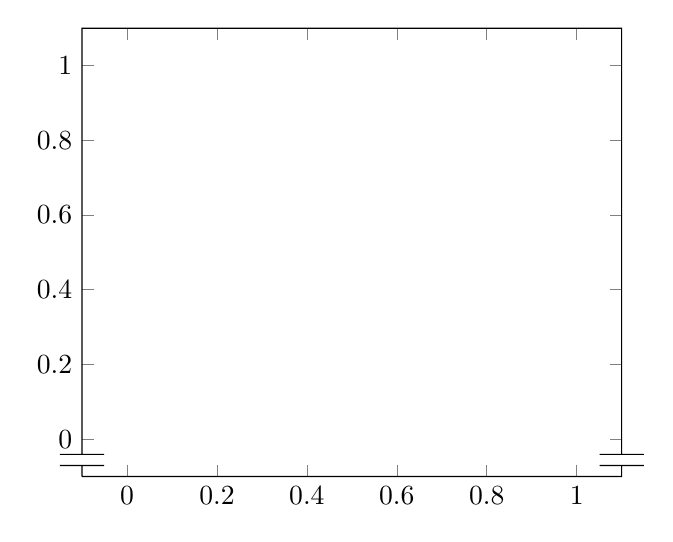
\begin{tikzpicture}
\begin{axis}[
	axis y discontinuity=parallel,
	]
	\smallplotstest
\end{axis}
\end{tikzpicture}
}

\AXISLINETESTS{closed axis lines}

{
\pgfplotsset{
	separate axis lines,
	axis line style={-stealth,thick},
	x axis line style={green},
	y axis line style={red}}

\AXISLINETESTS{Separate lines}
}
